\chapter*{Proposition 34}



\begin{figure*}[ht]
    \begin{center}
    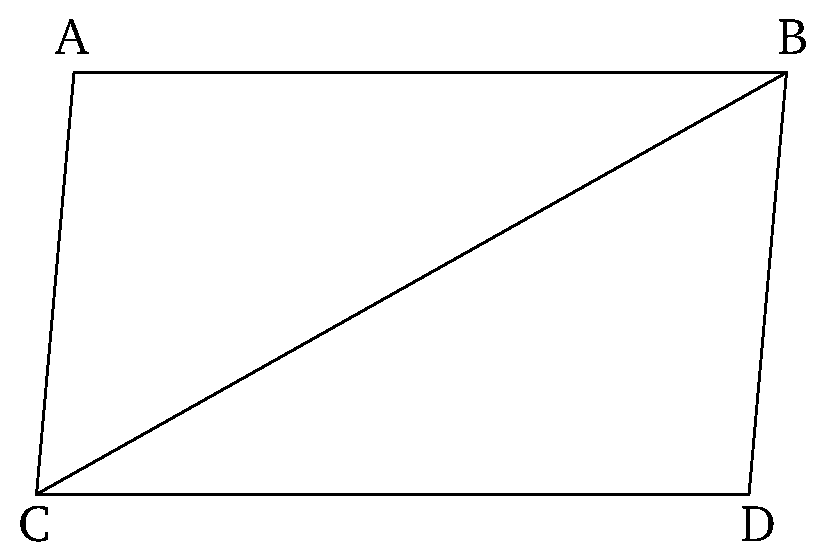
\includegraphics[width=0.5\linewidth]{figures/fig34e.eps}
    \label{fig:prop_34}
    \end{center}
\end{figure*}

In parallelogrammic figures the opposite sides and angles are equal to one
another, and a diagonal cuts them in half.\\

Let $ACDB$ be a parallelogrammic figure, and $BC$ its diagonal. I say that
for parallelogram $ACDB$, the opposite sides and angles are equal to
one another, and the diagonal $BC$ cuts it in half.

For since $AB$ is parallel to $CD$, and the straight-line $BC$ has fallen
across  them, the alternate angles $ABC$ and $BCD$ are equal to one another [Prop.~1.29]. 
Again, since $AC$ is parallel to $BD$, and $BC$ has fallen across them, the
alternate angles $ACB$ and $CBD$ are equal to one another [Prop.~1.29]. 
So $ABC$ and $BCD$ are two triangles having the two angles $ABC$ and
$BCA$ equal to the two (angles) $BCD$ and $CBD$, respectively, and one
side equal to one side---the (one) by the equal angles and common to them, (namely) $BC$. Thus,
they will also  have the remaining sides  equal to the corresponding
remaining (sides), and the remaining angle (equal) to the remaining angle [Prop.~1.26].
Thus, side $AB$ is equal to $CD$, and $AC$ to $BD$. Furthermore, angle $BAC$ is 
equal to $CDB$. And since angle $ABC$ is equal to $BCD$, and $CBD$ to
$ACB$, the whole (angle) $ABD$ is thus equal to the whole (angle) $ACD$.
And  $BAC$ was also shown  (to be) equal to $CDB$.

Thus, in parallelogrammic figures the opposite sides and angles are equal
to one another.

And, I also say that a diagonal cuts them in half. For since $AB$ is equal
to $CD$, and $BC$ (is) common, the two (straight-lines) $AB$, $BC$ are equal
to the two (straight-lines) $DC$, $CB$$^\dag$, respectively. And angle $ABC$ is
equal to angle $BCD$. Thus, the base $AC$ (is) also equal to $DB$, and
triangle $ABC$ is equal to triangle $BCD$ [Prop.~1.4].

Thus, the diagonal $BC$ cuts the parallelogram $ACDB$$^\ddag$ in half. (Which is) the
very thing it was required to show.


\section*{Commentary}

\begin{proposition}\label{proposition_34}\lean{Elements.Book1.proposition_34}\leanok
    If
\end{proposition}
\begin{proof}
    \uses{proposition_26,proposition_29}\leanok
\end{proof}
